% this file is called up by thesis.tex
% content in this file will be fed into the main document

\chapter[Genome architecture of the \emph{P. falciparum}
genome]{Three-dimensional modeling of the {\em P. falciparum} genome during
the erythrocytic cycle reveals a strong connection between genome
architecture and gene expression} % top level followed by section, subsection
\label{chap:plasmodium}

\graphicspath{{3_plasmodium/}}

\begin{work}

This chapter has been published in a slightly modified form in
\citep{ay:three-dimensional}, as joint work with Evelien Bunnik, Ferhat Ay,
Sebastiaan Bol, Jacques Prudhomme, Jean-Philippe Vert, Bill Noble and Karine
Le Roch.

\end{work}

\begin{abstract}{Résumé}

Dans ce projet, nous nous intéressons à l'architecture du parasite {\em
Plasmodium falciparum}, responsable de la forme la plus virulente et mortelle
du paludisme chez l'homme. Le développement de ce parasite est contrôlé par
des changements précis et coordonnés dans l'expression de ses gènes au cours
son cycle cellulaire. Les mécanismes régulant ces changements sont à l'heure
actuelle peu connus. Nous nous intéressons dans ce travail au lien entre
l'architecture spatiale du génome et la régulation des gènes.
Nous étudions la conformation du {\em P. falciparum} à trois moments de
son cycle cellulaire asexué érythrocyte (cycle cellulaire du parasite lors de
sa présence dans les cellules sanguines humaines). Grâce au protocole de
capture de la conformation des chromosomes associé au séquençage haut débit,
nous obtenons des cartes haute résolution des fréquences de contact entre
paires
de loci, à partir desquelles nous construisons des structures consensus
tridimensionnelles pour chaque étape du développement cellulaire du parasite.
Nous observons dans ces modèles une forte colocalisation des centromères,
des télomères, de l'ADN ribosomal, ainsi que les gènes "virulence". Ces
contraintes conduisent à une architecture complexe du génome, qui ne peut être
simplement expliquée par un modèle de volume d'exclusion comme celui de la
levure. Par ailleurs, les cartes de contacts exhibent des domaines
particuliers à la position des clusters internes de gènes "virulence",
suggérant l'importance du rôle de ces gènes dans l'architecture du génome.
Lors de l'état trophozoite, à mi chemin dans le cycle erythrocytique alors que
le génome est très fortement transcrit, celui-ci adopte une conformation plus
ouverte, et les chromosomes interagissent plus entre eux. Nous observons de
plus que les gènes à proximité des centres répressifs
sous-télomériques sont sous-exprimés. Par ailleurs, la colocalisation de
groupes de gènes spécifiques au parasite, tels que des gènes impliqués dans
l'invasion des cellules sanguines humaines, ont des profils d'expression
proches. Toutes ces observations suggèrent une très forte association entre
l'organisation spatiale du génome de {\em P. falciparum} et l'expression de
ses gènes. Une meilleure compréhension des processus biologiques impliqués
dans la dynamique de la conformation du génome pourrait contribuer à la
découverte de nouvelles stratégies pour combattre le paludisme.
\end{abstract}


\begin{abstract}{Abstract}
The development of the human malaria parasite {\em Plasmodium falciparum} is
controlled by coordinated changes in gene expression throughout its complex
life cycle, but the corresponding regulatory mechanisms are incompletely
understood. To study the relationship between genome architecture and gene
regulation in {\em Plasmodium}, we assayed the genome architecture of {\em P.
falciparum} at three time points during its erythrocytic (asexual) cycle.
Using chromosome conformation capture coupled with next-generation sequencing
technology (Hi-C), we obtained high-resolution chromosomal contact maps, which
we then used to construct a consensus three-dimensional genome structure for
each time point. We observed strong clustering of centromeres, telomeres,
ribosomal DNA and virulence genes, resulting in a complex architecture that
cannot be explained by a simple volume exclusion model. Internal virulence
gene clusters exhibit domain-like structures in contact maps, suggesting that
they play an important role in the genome architecture. Midway during the
erythrocytic cycle, at the highly transcriptionally active trophozoite stage,
the genome adopts a more open chromatin structure with increased chromosomal
intermingling. In addition, we observed reduced expression of genes located in
spatial proximity to the repressive subtelomeric center, and colocalization of
distinct groups of parasite-specific genes with coordinated expression
profiles. Overall, our results are indicative of a strong association between
the {\em P. falciparum} spatial genome organization and gene expression.
Understanding the molecular processes involved in genome conformation dynamics
could contribute to the discovery of novel antimalarial strategies.
\end{abstract}

\section{Introduction}

Malaria remains a major contributor to the global burden of disease, with an
estimated 219 million infected individuals and 660,000 deaths annually
\citep{who:malaria}. One of the main limiting factors for the development of
novel therapies is our poor understanding of mechanisms regulating the
parasite's complex life cycle, which involves several distinct parasitic
stages in the human and mosquito hosts. Regulation of these developmental
stages is thought to be controlled by coordinated changes in gene expression.
In addition, virulence associated with the human malaria parasite, {\em
Plasmodium falciparum}, is known to be directly linked to the parasite's
ability to tightly control the expression of genes involved in antigenic
variations on the surface of infected red blood cells. Some progress has been
made in elucidating mechanisms controlling the expression of these virulence
genes \citep{duraisingh:heterochromatin, freitas-junior:telomeric}.
Furthermore, a limited number of putative sequence-specific transcription
factors has been identified in the parasite genome \citep{balaji:discovery,
coulson:comparative}, including 27 ApiAP2 plant-like TFs, and drastic changes
in chromatin structure related to transcriptional activity have been observed
throughout the parasite erythrocytic cycle \citep{ponts:nucleosome}. However,
general and specific mechanisms controlling the expression of the ~6,372
parasite genes remain poorly understood.

In higher eukaryotes, several analyses have emphasized the role of genome
architecture in regulating transcription. Compartmentalization of the nucleus,
chromatin loops and long-range interactions contribute to a complex regulatory
network \citep{homouz:3d, kalhor:genome,  lieberman-aiden:comprehensive,
dixon:topological}. In {\em P. falciparum}, little is known about the effect
of genome organization on gene expression. Recent data indicate that genes
involved in control of parasite virulence ({\em var} genes) are associated
with repressive centers at the nuclear periphery
\citep{duraisingh:heterochromatin, dzikowski:mechanisms,
lopez-rubio:genome-wide} and that ribosomal DNA gene clusters are also
colocalized \citep{mancio-silva:clustering, lemieux:genome-wide}. However, a
global picture of the nuclear architecture throughout the parasite
erythrocytic cycle progression and its role in transcriptional regulation is
not yet available.

Chromosome conformation capture coupled with next generation sequencing (Hi-C)
measures the population average frequency of contacts between pairs of DNA
fragments in 3D space and can be used to model the spatial architecture of the
genome \citep{lieberman-aiden:comprehensive, duan:three-dimensional, kalhor:genome}. Here,
we performed a variant of the Hi-C protocol, tethered conformation capture
\citep{kalhor:genome}, to model at 10 kb resolution the spatial organization
of the {\em P. falciparum} genome throughout its erythrocytic cycle. Our
results indicate that the {\em P. falciparum} genome is highly structured,
with strong colocalization of centromeres, telomeres, active rDNA genes and
virulence gene clusters. These virulence genes exhibit distinctive contact
patterns and may therefore contribute to establishing the three-dimensional
structure of the {\em P. falciparum} genome. We identified discrete
chromosomal territories during the early and late stages of the parasite
erythrocytic cycle, which are partially lost in the highly transcriptionally
active trophozoite stage. Global chromosome movements during the erythrocytic
cycle are coherent with levels of transcriptional activity during the
different stages, and the three-dimensional genome architecture shows strong
correlation with gene expression levels. Collectively, our results suggest
that the {\em P. falciparum} genome organization and gene expression are
strongly interconnected.

\section{Results}

\subsection{Assaying genome architecture of {\em P. falciparum} at three stages using Hi-C}


\begin{figure}[h]
\centering
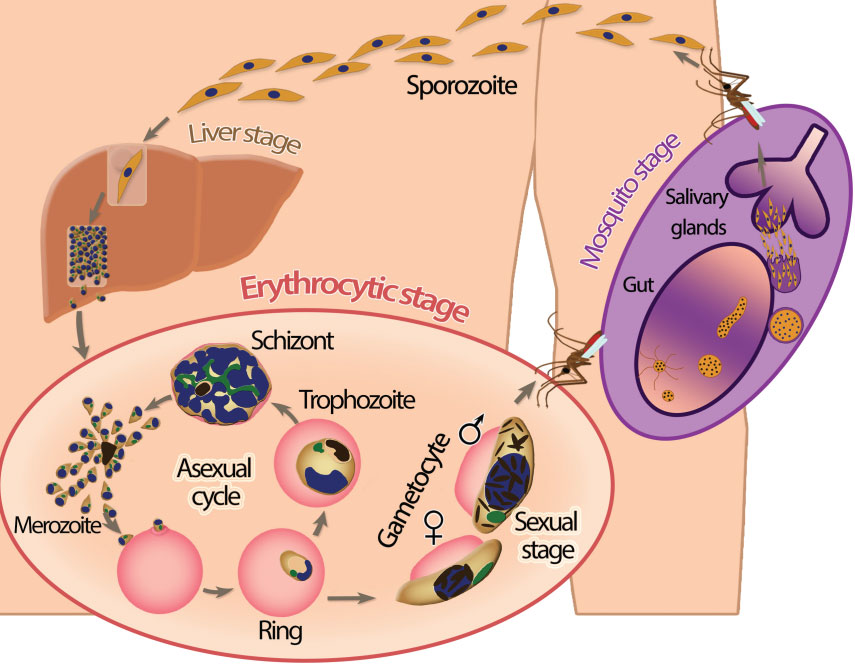
\includegraphics[width=\linewidth]{figures/fig1.pdf}
\caption{{\bf Tethered conformation capture of the {\em Plasmodium falciparum}
genome.}
\textbf{a,} Experimental protocol. \textbf{b,} Contact probability as a
function of genomic distance, with log-linear fits for the three erythrocytic
stages, as well as an experimental control. \textbf{c,} Normalized contact
count matrices at 10 kb resolution for chromosome 2 and chromosome 7 in the
schizont stage. \textbf{d,} Contact p-values (negative log10 scale) for
chromosome 2 and chromosome 7 in the schizont stage. In \textbf{(c)} and
\textbf{(d)}, yellow boxes denote clusters of VRSM genes, and blue dashed
lines indicate the centromere location.}
\label{fig:fig1}
\end{figure}



To study the genome architecture of {\em P. falciparum}, we harvested
parasites at three stages of the infected red blood cell cycle: after invasion
of red blood cells at the ring stage (0h), during high transcriptional
activity at the trophozoite stage (18h) and near the end of the cycle at the
schizont stage (36h), just before the newly formed parasites are released into
the bloodstream. Next, we applied the Hi-C protocol \citep{kalhor:genome} with
modifications to accommodate the extremely AT-rich genome of the malaria
parasite (Fig.~\ref{fig:fig1}a, Appendix Note 1, Appendix File 1).
As a control, we prepared a sample for which chromatin contacts were not
preserved by crosslinking of DNA and proteins.

We evaluated the quality of the resulting data for each sample. First, we
confirmed that the contact probability between two intrachromosomal loci
exhibits a log-linear decay with increasing genomic distance
(Fig.~\ref{fig:fig1}b, Appendix Fig.~\ref{suppfig:power-law}). Second,
we obtained lower numbers of interchromosomal contacts from crosslinked
samples relative to both random expectation and our control sample
(Appendix Table~\ref{table:ICP}). Third, we observed that the percentage
of long-range contacts (either interchromosomal or intrachromosomal $>$20 kb)
was significantly higher than control and comparable to the numbers observed
in yeast \citep{duan:three-dimensional} (Appendix Table~\ref{table:ICP}). Together,
these results indicated that we successfully assayed the {\em P. falciparum}
genome architecture with a high signal-to-noise ratio. We then coalesced the
mapped read pairs into a raw contact count matrix at 10 kb resolution, and we
corrected for potential technical and experimental biases
\citep{imakaev:iterative} (Fig.~\ref{fig:fig1}c, Appendix
Fig.~\ref{suppfig:ICE}) . The resulting normalized contact maps were used to
identify a subset of high-confidence contacts for each stage (Methods,
Appendix Note 2, Appendix File 2)~\citep{ay:statistical}. We
identified pairs of genes that show evidence of stage-specific contacts
(Methods) and then applied gene set enrichment analysis to the set of genes
that participate in such contacts.  This analysis identified significant
enrichment of VRSM genes for the ring and trophozoite stages (Appendix
Table~\ref{table:GSEAcompareStages}). This observation suggests that the
proximity between some VRSM clusters changes from the ring to trophozoite
stages, even though both stages show overall colocalization of VRSM clusters.
A similar enrichment analysis conducted using contacts that are specific to
two out of three stages resulted in no significant enrichment due to the small
number of genes involved in such contacts.

Normalized contact count and confidence score matrices exhibit a canonical
``X'' shape, indicative of a folded chromosome architecture anchored at the
centromere, as previously observed in yeast \citep{duan:three-dimensional,
tanizawa:mapping} and the bacterium {\em C. crescentus}
\citep{umbarger:three-dimensional} (Fig.~\ref{fig:fig1}c-d, Appendix
Fig.~\ref{suppfig:perChrFigs}). However, chromosomes that harbor
non-subtelomeric clusters of genes involved in antigenic variation and immune
evasion (Appendix File 3; VRSM genes: {\em var}, {\em rifin}, {\em
stevor} and {\em Pfmc-2tm})---chromosomes 4, 6, 7, 8 and 12---exhibit
additional folding structure (Fig.~\ref{fig:fig1}c-d, Appendix
Fig.~\ref{suppfig:perChrFigs}).

\subsection{Three-dimensional modeling recapitulates known organizational principles of {\em Plasmodium} genome}

\begin{figure}[h]
\centering
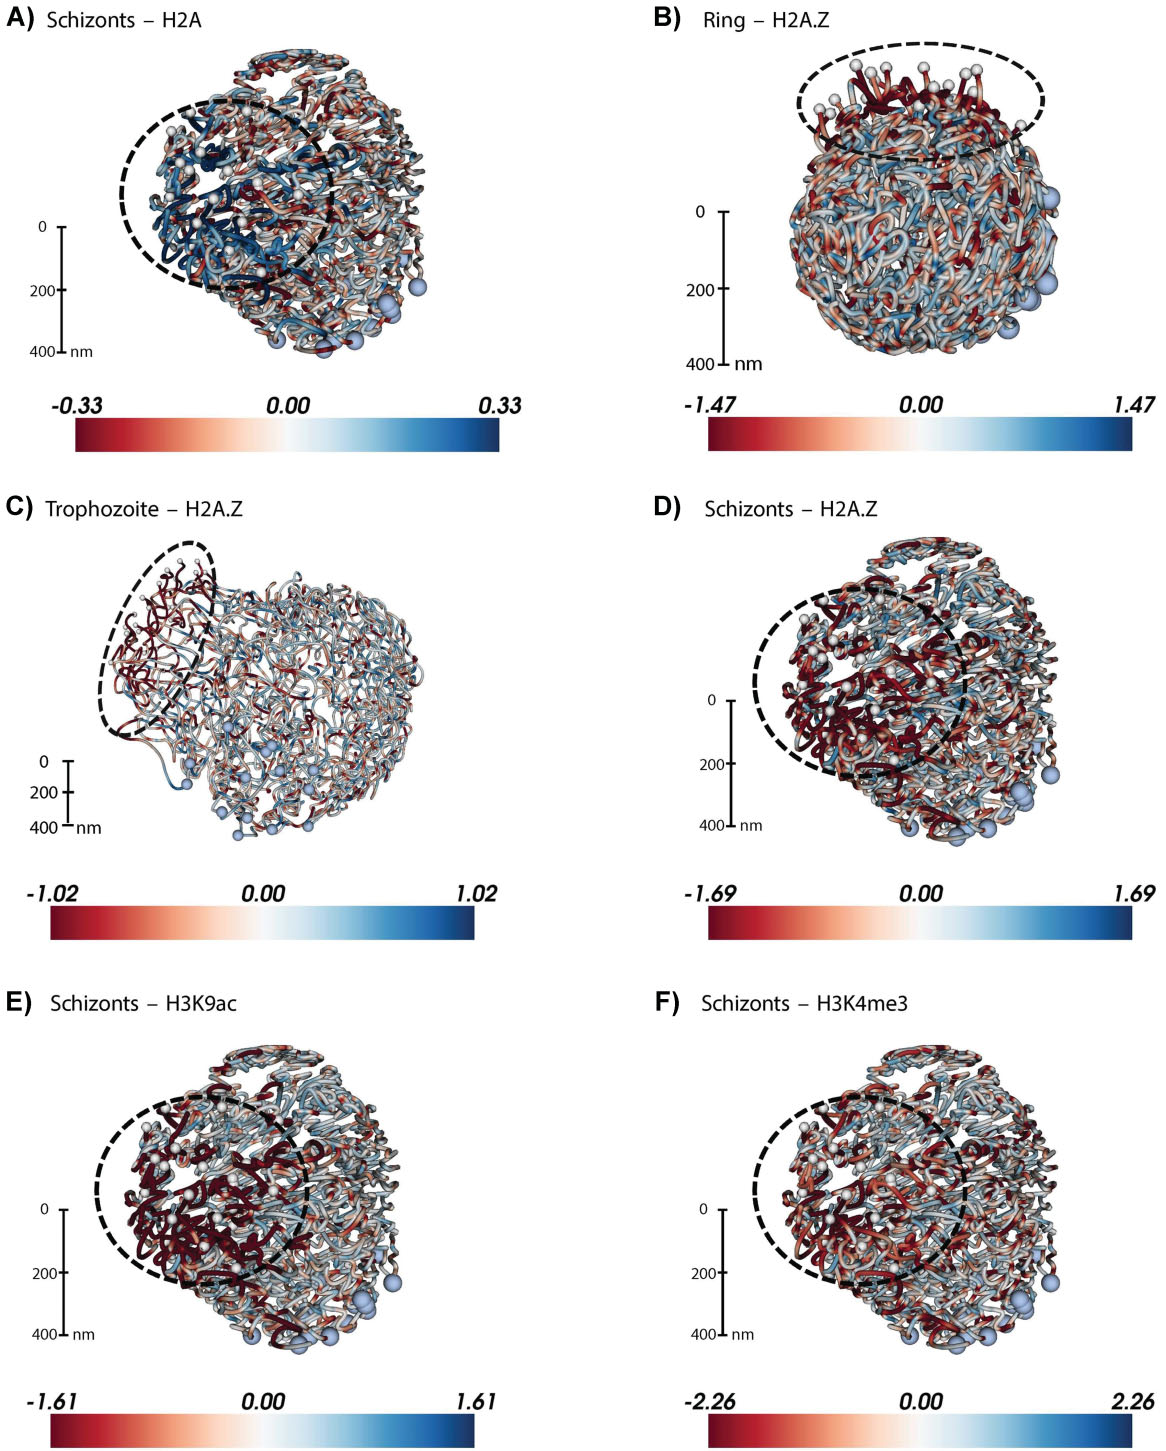
\includegraphics[width=\linewidth]{figures/fig2.pdf}
\caption{{\bf 3D modeling and validation with DNA FISH.}
 \textbf{a,} 3D structures of all three stages. The nuclear radii used to
 model ring, trophozoite and schizont stages were 350, 850, and 425 nm,
 respectively. Centromeres and telomeres are indicated with light blue and
 white spheres, respectively. Midpoints of VRSM gene clusters are shown with
 green spheres. \textbf{b,} Validation of colocalization between a pair of
 interchromosomal loci with VRSM genes (chr7: 550,000 - 560,000 that harbors
 internal VRSM genes and chr8: 40,000 - 50,000 that harbors subtelomeric VRSM
 genes) by DNA FISH (left) and by the three-dimensional model for the
 corresponding stage (right). The location of the loci in the 3D model is
 indicated with light blue spheres and pointed by black arrows. \textbf{c,}
 Validation same as in \textbf{(b)} for a pair of interchromosomal loci that
 harbor no VRSM genes (chr7: 810,000 - 820,000 and chr11: 820,000 - 830,000).
 }
 \label{fig:fig2}
 \end{figure}




To better characterize the genome architecture, we generated for each stage
100 consensus 3D structures, each of which summarizes the population average
(Fig.~\ref{fig:fig2}a, Methods), using multidimensional scaling (MDS) with two
primary constraints \citep{duan:three-dimensional}: (i) the DNA must lie within a sphere
with a specified diameter \citep{bannister:making, weiner:3d} and (ii)
adjacent 10kb loci must not be separated by more than 91 nm
\citep{bystricky:long-range}. \emph{P. falciparum} undergoes an atypical form
of cell division, resulting in schizont stage parasites with multiple
independent nuclei, each containing 1n chromosomes. Note that our model
assumes that a single copy of each chromosome is present in each structure,
thus averaging the signal from these multiple nuclei per cell.


We performed a series of experiments to assess the robustness of our 3D
inference procedure.  Our results showed only slight changes in the inferred
3D models when we varied the parameter used in conversion of contact counts to
expected distances (Appendix Table~\ref{table:stabilityToBeta}). This
was also true when we removed from the inference the two types of spatial
constraints related to nuclear volume and to distances between adjacent beads
(Appendix Table~\ref{table:stabilityToConstraints}). Finally, our
experiments on the impact of the initialization step (Methods) showed that
structures inferred from different initial configurations are highly similar
(Appendix Fig.~\ref{suppfig:compareStructurePairs}), do not fall into
discrete clusters (Appendix Fig.~\ref{suppfig:CHindices}) and all such
structures exhibit common organizational hallmarks (Appendix
Fig.~\ref{suppfig:clusteringIn100Structures}). Because of the stability of
our inference procedure, hereafter we generally present and discuss the
results for only one representative structure per stage.

Although the modeling procedure contains no explicit constraints on telomere
or centromere locations, we observe strong colocalization of both sets of loci
across all three stages (Fig.~\ref{fig:fig2}a, Appendix
Fig.~\ref{suppfig:3Dcentromeres}, Appendix Table~\ref{table:witten}),
with centromeres and telomeres localizing in distal regions of the nucleus. To
understand further the colocalization patterns of centromeres and telomeres in
each stage, we divided each chromosome into three compartments
(left--mid--right or telomeric--centromeric--telomeric) using eigenvalue
decomposition (Methods) and then performed hierarchical clustering on the
matrix of pairwise distances between compartments (Appendix
Fig.~\ref{suppfig:compDists}). At each stage, we observed clusters that are
comprised primarily of either centromeric or telomeric compartments. In
particular, during the trophozoite stage, all the centromeric compartments
fall into two main clusters suggesting strong colocalization of all
centromeres for this stage (Appendix Fig.~\ref{suppfig:compDists}d).
Such strong colocalization has previously been observed by immunofluoresence
microscopy at the trophozoite and schizont stages but not at the early ring
stage \citep{hoeijmakers:plasmodium}. However, when the size of the nucleus is
used as a marker of the parasite asexual cycle stage \citep{bannister:making,
weiner:3d}, the cells that are presented as trophozoites in this previous
study \citep{hoeijmakers:plasmodium} are more similar to our ring stage
parasites, indicating that centromere clustering also occurs early in the
erythrocytic cycle. Furthermore, if the centromeres are stochastically
distributed between a small number of foci within a population, then an assay
that measures average signal, such as Hi-C, will indeed demonstrate an
aggregate clustering for the centromeres and not complete dispersion as
suggested by a recent study \citep{lemieux:genome-wide}. These results suggest
that {\em P. falciparum} nuclei are highly structured around centromeres and
telomeres, consistent with known organizational principles gathered through
multiple independent microscopy experiments \citep{duraisingh:heterochromatin,
dzikowski:mechanisms, lopez-rubio:genome-wide, hoeijmakers:plasmodium}.


\subsection{Virulence gene clusters on different chromosomes colocalize in 3D}

In addition to centromeres and telomeres, we observed for all VRSM gene
clusters, both internal and subtelomeric, a significant colocalization with
one another (Fig.~\ref{fig:fig2}a, Appendix Table~\ref{table:witten}).
The significant colocalization for VRSM clusters as well as for centromeres
and telomeres were all reproducible when we used contact counts instead of 3D
distances to perform colocalization tests similar to Appendix
Table~\ref{table:witten} (data not shown). Given colocalization of the
telomeres, colocalization of subtelomeric clusters is not surprising. However,
the proximity of internal VRSM clusters with one another and with subtelomeric
clusters is unexpected under the random polymer looping model and, to the best
of our knowledge, observed experimentally for the first time. To further
validate these results inferred from our 3D models, we performed DNA
fluorescence {\em in situ} hybridization (FISH) (Methods, Appendix Note
3) on an interchromosomal pair of strongly interacting (at 10 kb resolution)
VRSM clusters: the internal cluster from chromosome 7 and a subtelomeric
cluster from chromosome 8. We observed strong colocalization by FISH ($>$90\%
of cells, Fig.~\ref{fig:fig2}b, Appendix Fig.~\ref{suppfig:fish}a,
Appendix Table~\ref{table:FISHprimers}), providing independent support
for the clustering of VRSM genes. Although previous FISH results indicated
that {\em var} genes form 2 to 5 clusters in 3D per cell
\citep{freitas-junior:frequent, lopez-rubio:genome-wide}, others recently
showed single foci for the VRSM gene-associated repressive histone mark
H3K9me3 and heterochromatin protein 1 (PfHP1) \citep{dahan:pfsec13}, as well
as for H3K36me3 that marks both active and silenced {\em var} genes
\citep{ukaegbu:recruitment}. Because our experimental strategy (Hi-C) captures
a population average, we are unable to distinguish between multiple VRSM gene
clusters in 3D if the genes are randomly distributed among clusters from cell
to cell. Using FISH experiments, we also observed strong colocalization
($>$90\% of cells, Fig.~\ref{fig:fig2}c, Appendix
Fig.~\ref{suppfig:fish}b) for a pair of interchromosomal loci located outside
VRSM clusters with consistent strong interactions at all three stages, while
colocalization was not observed for a pair of non-interacting interchromosomal
loci ($<$10\% of cells, Appendix Fig.~\ref{suppfig:fish}c). These
results demonstrate that our population average Hi-C data agrees with a
majority of single cell FISH images.

\subsection{Highly transcribed rDNA units colocalize in 3D during the ring stage}

 
 \begin{figure}[h]
 \centering
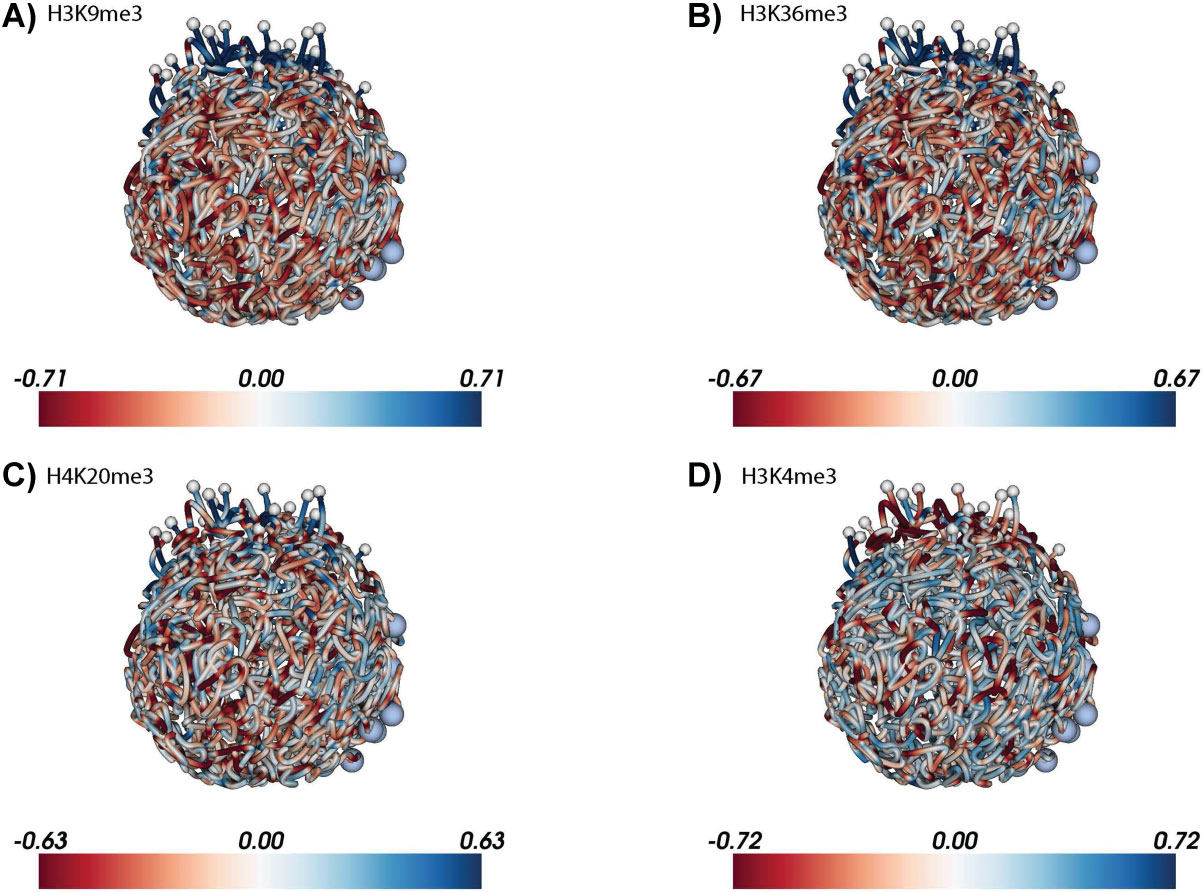
\includegraphics[width=\linewidth]{figures/fig3.pdf}

 \caption{{\bf Colocalization of highly transcribed rDNA units.} 
  Virtual 4C plots generated at 25 kb resolution using as a bait the A-type
  rDNA unit on chromosome 7 from crosslinked Hi-C libraries of \textbf{(a)}
  ring, \textbf{(b)} trophozoite, \textbf{(c)} schizont stages and
  \textbf{(d)} from the trophozoite control library. Vertical red line
  indicates the midpoint of the A-type rDNA unit on chromosome 5. Normalized
  contact counts from 50 kb up- and downstream of the 25 kb bin containing the
  rDNA unit are used, omitting the rDNA-containing window itself to exclude
  repetitive DNA. For each window $w$ on chromosome 5, the contact enrichment
  is calculated by dividing the contact count between the bait and $w$ to the
  average interchromosomal contact count for the bait locus.
  }
  \label{fig:fig3}
  \end{figure}



Similar to VRSM genes, the rDNA genes are strictly regulated during the
parasite life cycle. In {\em P. falciparum}, these genes are dispersed on
different chromosomes in five rDNA units containing the 18S, 5.8S and 28S
genes and one repeat unit consisting of three copies of the 5S gene. A
previous FISH study suggested that all rDNA units localize at a single
nucleolus but also claimed that the two units on chromosomes 5 and 7 that are
actively transcribed during the ring stage (A-type units) are dispersed in the
ring stage \citep{mancio-silva:clustering}. However, a more recent Hi-C study
of ring stage parasites demonstrated strong clustering of these two A-type
units in multiple strains \citep{lemieux:genome-wide}. Analysis of our Hi-C
data confirmed overall enrichment of contacts between chromosomes 5 and 7 in
all three stages and showed a particular peak of enrichment centered at the
rDNA unit on chromosome 5 among all interchromosomal contact partners of the
rDNA unit on chromosome 7 in the ring stage (3.32x, Fig.~\ref{fig:fig3}a). We
observed less striking enrichment of contacts that are not specific to or
centered on the rDNA units for the other two stages (trophozoites (1.99x),
schizonts (1.23x), Fig.~\ref{fig:fig3}b-c) during which the two rDNA units are
not transcribed \citep{mancio-silva:clustering}. Reanalysis of the Lemieux
{\em et al.} data using our processing pipeline also showed this enrichment
consistently in three different NF54-derived strains in the ring stage (6.06x,
4.47x and 4.61x, respectively, Appendix
Fig.~\ref{suppfig:rDNAunitsOn3D}a-c). Control libraries from both studies do
not exhibit this enrichment (Fig.~\ref{fig:fig3}d, Appendix
Fig.~\ref{suppfig:rDNAunitsOn3D}d). Our 3D models for the ring stage place
these two A-type rDNA units near the nuclear periphery. Together with the
strong colocalization between A-type rDNA, these results suggest the existence
of perinuclear transcriptionally active compartments. Such compartments may
play a role in separating out the single active var gene per cell from compact
chromatin around (sub)telomeric regions marked by the repressive H3K9me3
modification \citep{lopez-rubio:genome-wide}. We did not observe an overall
colocalization between all rDNA units in the ring stage, including the three
18S, 5.8S, 28S units and one 5S unit that are not expressed during asexual
erythrocytic cycle (Appendix Table~\ref{table:witten}).  This
observation suggests that genomic location may influence rDNA expression by
the preferential colocalization of the expressed rDNA units, away from the
non-expressed units.

\subsection{Transcriptionally active trophozoite stage exhibits an open chromatin structure}

Assaying three different time points, we observed significant changes in
chromatin structure throughout the erythrocytic cycle. To visualize high-level
changes, we generated animations showing the movement of chromosomes as the
parasite progresses through its cell cycle (Appendix Files 4-18). We then
characterized global chromatin changes by analyzing the relationship between
contact frequency and genomic distance (Fig.~\ref{fig:fig1}b, Appendix
Fig.~\ref{suppfig:power-law}). The gradient of the log-linear fit is very
close to -1 in both the ring and schizont stages (-0.98 and -0.96,
respectively) indicative of a fractal globule genome architecture that is
usually found in higher eukaryotes \citep{lieberman-aiden:comprehensive}.
Intriguingly, the intermediate and most active transcriptional stage yields a
log-linear fit value with gradient -1.14, a value between the fractal (-1) and
the equilibrium globule (-1.5) model suggested in yeast
\citep{fudenberg:higher-order} and indicative of more chromosomal
intermingling. Indeed, a value of -1.17 has been demonstrated to correspond to
a state of ``unentangled rings'' similar to the fractal globule state, in
which the rings may correspond to long chromosomal regions looped on or
anchored to a nuclear scaffold \citep{vettorel:statistics}. It is important to
note that the value of the gradient is determined solely by Hi-C contact
counts and,  therefore, the above mentioned difference is independent of our
3D modeling and the change in the nuclear radius from one stage to another.
Furthermore, the difference in the gradient value for trophozoites compared to
the two other stages is consistent for each chromosome, suggesting that all
chromosomes change their folding behavior during the trophozoite stage
(Appendix Table~\ref{table:scalingFactors}).

In order to further investigate whether trophozoites show a more open
chromatin structure than the two other stages, we systematically compared our
data across all three stages. First, we computed and compared intra and
interchromosomal contact probabilities for each stage (Appendix
Fig.~\ref{suppfig:intraVSinter}). We observed that intrachromosomal contacts,
even at very large distances, are more prevalent than interchromosomal
contacts for all three stages, suggesting the existence and preservation of
chromosome territories throughout the erythrocytic cycle. However, the
enrichment in intrachromosomal contacts was the lowest for trophozoite stage
for distances above 300~kb, suggesting a relative loss of territories in this
stage compared to the other two. Second, we quantified how preserved the
chromosomal territories are at each stage by estimating the degree of
chromosome intermingling in our 3D models. We randomly sampled small spheres
in the nucleus and asked, for each chromosome {\em i}, what percentage of the
spheres that contain any locus from chromosome {\em i} also contain a locus
from another chromosome {\em j}. Our results using different sphere sizes, and
controlling for the varying nuclear diameter, consistently exhibited the
highest amount of intermingling for the trophozoite stage and the highest
territory preservation for the schizont stage (Appendix
Fig.~\ref{suppfig:territory}).

To understand the architectural dynamics responsible for the systematic
changes in chromatin compaction, we computed the relative movements among
chromosome compartments during the erythrocytic cycle. Despite the increase in
nuclear volume, many interchromosomal compartment pairs came closer together
in the transition from the ring to trophozoite stage (Appendix
Fig.~\ref{suppfig:compMovement}a, red color). Subsequently, most
interchromosomal compartments moved away from each other in the transition to
the schizont stage (Appendix Fig.~\ref{suppfig:compMovement}b, blue
color), resulting in more compact chromatin that favors formation of
chromosome territories. These results are consistent with a previously
proposed model, in which the {\em P. falciparum} nucleus exhibits a more open
chromatin configuration at the trophozoite stage, enabling interchromosomal
contacts and high levels of transcriptional activity \citep{ponts:nucleosome}.

\subsection{{\em Plasmodium} genome architecture cannot be explained by volume exclusion}


  \begin{figure}[h]
  \centering
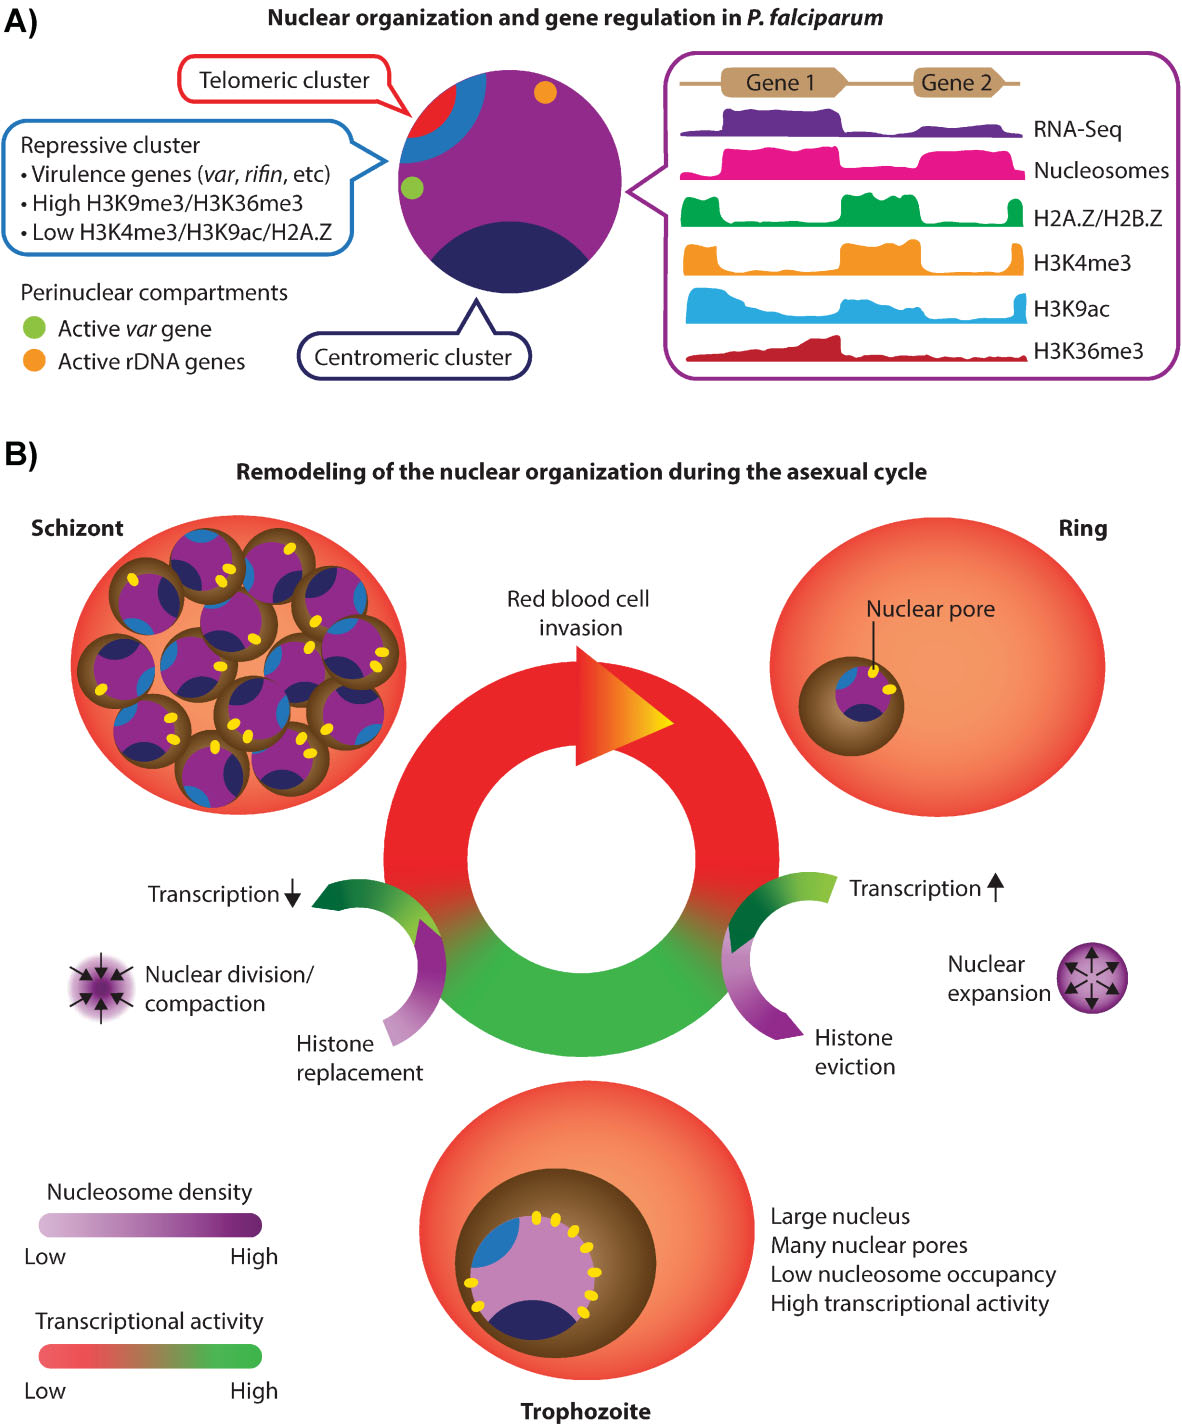
\includegraphics[width=\linewidth]{figures/fig4.pdf}
  \caption{{\bf Volume exclusion modeling. }
  Observed/expected contact frequency matrices illustrate, for each locus,
  either the depletion (blue) or enrichment (red) of interaction frequencies
  compared to what would be expected given their genomic distances.
  \textbf{a,} Observed/expected contact frequency matrices derived from {\em
  S. cerevisiae} chr 7 from volume exclusion modeling (left) and Hi-C data
  (right). \textbf{b,} Observed/expected matrices from volume exclusion
  modeling (left) and Hi-C data (right) for {\em P. falciparum} chr 7 during
  the trophozoite stage.}
  \label{fig:fig4}
  \end{figure}



We next assessed whether the primary architectural features in {\em P.
falciparum} arise from a population of constrained but otherwise random
configurations of chromatin following a simple volume exclusion (VE) model, as
recently shown for {\em Saccharomyces cerevisiae} \citep{tjong:physical}. We
therefore repeated the Tjong {\em et al.} simulations using the same set of
constraints and successfully recovered the strong correlation between the
simulated map and the experimentally observed yeast contact map (raw
correlation of 0.91; normalized correlation of 0.57; Fig.~\ref{fig:fig4}a,
Methods, Appendix Note 4, Appendix
Fig.~\ref{suppfig:VEconvergence}). In contrast, our simulations for the ring,
trophozoite and schizont stages of {\em P. falciparum} yielded markedly lower
correlations (normalized correlation of 0.34, 0.39 and 0.49, respectively) and
strikingly different contact maps compared to the experimentally observed maps
(Fig.~\ref{fig:fig4}b). One significant reason for the observed discrepancy
between yeast and {\em P. falciparum} is the lack of structure around clusters
of VSRM genes in the simulated data (Fig.~\ref{fig:fig4}b). Accordingly, we
conclude that the simple volume exclusion model, which so convincingly
explains the yeast genome architecture, is insufficient to explain the
observed architecture of {\em P. falciparum} genome, highlighting the need for
a genome-wide assay such as Hi-C to obtain accurate structural models.

\subsection{VRSM gene clusters form domain-like structures}

  \begin{figure}[h]
\includegraphics[width=\linewidth]{figures/fig5.pdf}
  \centering
  \caption{{\bf Role of internal VRSM gene clusters in shaping genome
  architecture.}
   \textbf{a-d,} Heatmaps of scaled pairwise Euclidean distances derived from
   the 3D model at 10 kb resolution for \textbf{(a, b)} two chromosomes that
   harbor internal VRSM gene clusters and \textbf{(c, d)} two chromosomes that
   do not. Yellow boxes indicate locations of VRSM clusters. }
   \label{fig:fig5}
   \end{figure}



Our results from the volume exclusion modeling and from visual inspection of
the contact maps suggest that the internal VRSM gene clusters are associated
with distinctive structural features. All eight of the internal VRSM clusters
induce a striking cross-like shape, both in the contact count and 3D distance
matrices (Fig.~\ref{fig:fig5}a-b, Appendix
Fig.~\ref{suppfig:perChrFigs}). Quantification of this phenomenon revealed a
consistent contact pattern across all eight internal VRSM clusters
(Appendix Fig.~\ref{suppfig:TADs}), suggesting that VRSM gene clusters
adopt a compact, domain-like structure. Although these domain-like structures
resemble topologically associated domains (TADs) described in mammals
\citep{dixon:topological, nora:spatial}, the VSRM domains are much smaller
(10--50 kb) compared to TADs (0.1--1 Mb). Furthermore, because VRSM genes have
no orthologs in human and mouse, mechanisms regulating these domain-like
structures likely differ from the one in mammalian genomes. Further
understanding of how these VRSM domains are formed in  \emph{Plasmodium} would
shed light on genome architecture associated regulation of VRSM gene
expression.

Another interesting pattern involving internal VRSM clusters emerged from
further inspection of chromosome compartments.  Five of the eight internal
VRSM clusters (two on chromosome 4, one on chromosome 7 and both clusters on
chromosome 12) occur at compartment boundaries (third and fourth rows of
Appendix Fig.~\ref{suppfig:perChrFigs}). This striking overlap  suggests
that VRSM genes may contribute to or rely upon the boundaries of chromosomal
compartments. Taken together with the domain-like structures around these VRSM
clusters, these results confirm that genome architecture is likely to be
involved in the strict regulation of virulence genes during the erythrocytic
cycle.

\subsection{Expression is highly concordant with 3D localization for {\em Plasmodium} genes}

\begin{figure}[h]
\includegraphics[width=\linewidth]{figures/fig6.pdf}
\centering
\caption{{\bf Relationship between 3D architecture and gene expression.}
\textbf{a,}Correlation between expression profiles of pairs of
interchromosomal genes as a function of number of contacts linking the two
genes. To generate this plot all interchromosomal gene pairs are first sorted
in increasing order of their expression correlation and then binned into 20
equal width quantiles ($5$th, $10$th, ..., $100$th). For each bin, the average
expression correlation between gene pairs (x-axis) and the average normalized
contact count linking the genes in each pair together with its standard error
(y-axis) are computed and plotted. Interchromosomal gene pairs that have
contact counts within the top 20\% for each stage have more highly correlated
expression profiles than the remaining gene pairs [Wilcoxon rank-sum test,
p-values 2.48e-206 (ring), 0 (trophozoite), and 0 (schizont)].
\textbf{b,} Correlation between expression profiles of pairs of
interchromosomal genes as a function of 3D distance between the genes. This
plot is generated similar to \textbf{a} but with using 3D distances instead of
contact counts (y-axis). In order to summarize results from multiple 3D
structures per each stage, we plot the median value among 100 structures with
a red line and shaded the region corresponding to the interval between 5th and
95th percentile with gray. Interchromosomal gene pairs closer than 20\% of the
nuclear diameter have more highly correlated expression profiles than genes
that are far apart [Wilcoxon rank-sum test, p-values 7.17e-221 (ring), 0
(trophozoite), and 1.57e-88 (schizont)].
\textbf{c,} Gene expression as a function of distance to telomeres. To
generate this plot all genes are first sorted by increasing distance to the
centroid of telomeres (x-axis) and then binned similar to \textbf{a} into 20
equal width quantiles. The average log expression
value~\citep{bunnik:polysome}
together with its standard error (y-axis) is plotted for genes in each bin. In
order to summarize results from multiple 3D structures per each stage, we plot
the median value among 100 structures with a red line and shaded the region
corresponding to the interval between 5th and 95th percentile with gray. Genes
that lie within 20\% of the nuclear diameter to the centroid of the telomeres
showed significantly lower expression levels [Wilcoxon rank-sum test, p-values
1.54e-12 (ring), 1.69e-32 (trophozoite), 3.37e-20 (schizont)].
\textbf{d,} First kCCA expression profile component score, corresponding to
the projection of the gene expression profile onto the extracted kCCA profile
for the trophozoite stage.}
\label{fig:fig6}
\end{figure}




Next, we investigated the relationship between the three-dimensional genome
structure and gene expression using four published expression data sets
\citep{leroch:discovery, lopez-barragan:directional, otto:new,
bunnik:polysome}. First, we observed that, for each of the three stages,
interchromosomal pairs of genes that strongly interact (contact counts within
the top 20\%) as well as gene pairs that are in close proximity ($<$20\% of
the nuclear diameter) showed more correlated expression profiles than genes
that are far apart (Fig.~\ref{fig:fig6}a,b), as previously observed in yeast
\citep{homouz:3d}. To assess whether these observed trends are confounded by
similarly expressed VRSM genes that strongly interact with each other and are
placed together near telomeres by our 3D model, we repeated the above analyses
by excluding all VRSM genes (Appendix
Fig.~\ref{suppfig:expVSdistWithoutVRSM}). Even though the observed trends are
weakened by exclusion of VRSM genes, the decrease in 3D distance and increase
in contact count with increasing expression correlation remained significant
(Appendix Fig.~\ref{suppfig:expVSdistWithoutVRSM}). It is also important
to note that, for these analyses, we excluded intrachromosomal gene pairs to
only focus on the relationship between 3D proximity and gene expression by
eliminating the confounding effect caused by genes that lie nearby on a
chromosome and show similar expression profiles. Second, we analyzed gene
expression in relation to the repressive subtelomeric clusters
\citep{duraisingh:heterochromatin, dzikowski:mechanisms,
lopez-rubio:genome-wide} and other nuclear landmarks. The subset of genes that
lie within 20\% of the nuclear diameter to the centroid of the telomeres
showed significantly lower expression levels than more distal genes
(Fig.~\ref{fig:fig6}c). The repressive effect of the subtelomeric clusters is
apparent in all three stages and is strongest at the trophozoite stage, in
which subtelomeric VRSM clusters are known to be tightly repressed
\citep{chen:developmental}. If we remove the VRSM genes from the analysis, the
repressive effect is still significant at the trophozoite stage, which is
known to be the most active transcriptional stage of the erythrocytic cycle
(Appendix Fig.~\ref{suppfig:distToCenter}a,b). Similar analysis showed
higher expression levels for genes located near the nuclear center, as well as
for genes close to the centroid of the centromeres (Appendix
Fig.~\ref{suppfig:distToCenter}c,d). Furthermore, we observed significant and
consistent colocalization across all three stages for 11 of the 15 expression
clusters identified in \cite{leroch:discovery} (Appendix
Table~\ref{table:witten}). Strikingly, the trophozoite stage showed
significant colocalization for clusters associated with genes that are
repressed during this stage (clusters 1, 3, 4, and 13-15) as well as genes
that exhibit high levels of expression (clusters 6, 9, 10, and 12), confirming
the strong relationship between 3D location and gene expression.

To further explore the relationship between gene expression and 3D structure,
we employed an unsupervised learning method known as {\em kernel canonical
correlation analysis} (kCCA) \citep{bach:kernel}. This methodology identifies
a set of orthogonal gene expression profiles that exhibit coherence with
respect to the 3D structure (Methods). For all stages, the projection of gene
expression patterns onto the first extracted profile exhibits a striking
transcriptional gradient across the 3D structure, from the telomere cluster to
the opposite side of the nucleus  (Fig.~\ref{fig:fig6}c, Appendix
Fig.~\ref{suppfig:kCCAsecond}a,c,e). The coherence with 3D structure drops
significantly in the second component of the kCCA (Appendix
Fig.~\ref{suppfig:kCCAsecond}b,d,f), suggesting that gene expression is
strongly influenced by distance to the subtelomeric repressive center. To
further interpret the kCCA results we employed gene set enrichment analysis
\citep{subramanian:gene} on the ranked lists of projections onto the first
kCCA component. The results showed, for all three stages, significant
enrichment (q-value $<$ 0.01) of gene sets related to antigenic variation and
translation (i.e. ribosome proteins) on the telomeric and non-telomeric side,
respectively, of the extracted kCCA expression profile (Appendix
Tables~\ref{table:RingsFirstPro},~\ref{table:TrophsFirstPro},~\ref{table:SchizontsFirstPro}).
Similar to the colocalization test results for expression clusters of
\cite{leroch:discovery}, clusters of genes that are repressed (clusters 4, 13,
and 14) and expressed (clusters 6 and 9-12) in the trophozoite stage showed
consistent enrichment in the strongest kCCA profile (Appendix
Table~\ref{table:kCCAforClusters}). In addition, genes exclusively expressed
in sporozoites (cluster 1) and gametocytes (clusters 3) were also strongly
enriched, indicating that the repression of these genes during the asexual
erythrocytic cell cycle may be related to their localization within the
nucleus. Finally, for GO terms related to parasite invasion (rhoptry, myosin
complex, motor activity; q-value $<$ 0.1) and for the cluster of invasion
genes (cluster 15), we observed an enrichment relative to the second kCCA
component, suggesting that expression of invasion genes may also be regulated
by the 3D genome structure (Appendix
Tables~\ref{table:kCCAforClusters},~\ref{table:secondPro}).


\section{Discussion}

This study presents the first analysis of genome architecture during the cell
cycle of a eukaryotic pathogen. Overall, our data demonstrate that the genome
of {\em P. falciparum} exhibits a higher degree of organization than the
similarly sized budding yeast genome. Although localization of chromosomes
within the {\em P. falciparum} nucleus is partially dictated by size
constraints, the simple volume exclusion model observed in yeast is
insufficient to explain the 3D architecture of the {\em P. falciparum} genome.
In particular, a striking spatial complexity is added by clusters of virulence
genes, which function as critical structural elements that shape the genome
architecture. Furthermore, our model correlates well with expression levels of
parasite-specific gene sets and shows strong clustering of repressed genes and
highly transcribed rDNA units, indicative of a non-random genomic organization
that contributes to gene regulation during the asexual erythrocytic cycle.
Considering the strong association between nuclear architecture and gene
expression as well as the observed domain-like structures, {\em Plasmodium}
species may be excellent model organisms to study the impact of genome
structure on gene regulation. The lower complexity of genome organization in
organisms with similarly sized genomes, such as yeast, may indeed be less
informative for such investigations.

Assaying multiple time points during the parasite's erythrocytic cycle
revealed intriguing changes in genome structure between the different
developmental stages. Our results show that the genome adopts a more open
conformation during the trophozoite stage consistent with high transcriptional
activity in this stage of the erythrocytic cycle, followed by compaction of
chromosomes into discrete chromosome territories before re-invasion of a new
host cell. A similar pattern was observed previously for nucleosome occupancy,
with strong histone depletion at the trophozoite stage and nucleosome
replacement at the schizont stage \citep{ponts:nucleosome}. Based on these
observations, we hypothesize that the spatial genome organization of {\em P.
falciparum}, coupled with its dynamic chromatin structure, acts as an
important alternative mechanism of transcriptional regulation, possibly
compensating for the lack of a diverse collection of specific transcription
factors \citep{balaji:discovery, coulson:comparative} and the low capacity of
the parasite to regulate gene expression in response to metabolic stress
\citep{ganesan:genetically, leroch:systematic}. These changes in genome
architecture could mainly be indicative of differences between the various
developmental stages of the parasite, but could also be related to cell cycle
progression itself. Given the importance of nuclear architecture for
regulation of gene expression, disruption of its genome organization is likely
to interfere with parasite development through the erythrocytic cycle and
could therefore be lethal to the parasite. Compounds targeting proteins
involved in establishing and maintaining the three-dimensional genome
structure in {\em P. falciparum} may thus have potent antimalarial activity.

A recently published Hi-C study suggested that chromosomal territories are
absent in the ring stage parasites, especially for larger chromosomes
\citep{lemieux:genome-wide}. In contrast, our data provides multiple lines of
evidence for the existence of chromosome territories throughout the
erythrocytic cell cycle. In particular, we observed that intrachromosomal
contacts, even at very large distances, are more prevalent than
interchromosomal contacts. This observation is supported by our own Hi-C data
in three stages as well as by our reanalysis of the Lemieux {\em et al.} data
(Appendix Fig.~\ref{suppfig:intraVSinter}b-e). The difference between
the two analyses can be traced to our improved method for discretizing the
genomic distance axis, which avoids bins with few observations and, hence,
high variance (Appendix Fig.~\ref{suppfig:intraVSinter}a versus b). Even
though further experiments may be necessary to reconcile these differences,
our results strongly suggest that {\em P. falciparum} chromosomes occupy
distinct territories, similar to other eukaryotic genomes.

Clustering of virulence gene families into a distinct nuclear compartment is
likely to play an important role in the formation of repressive
heterochromatin that controls the silencing of these genes. Heterochromatin
around virulence genes is characterized by histone modifications H3K36me3
\citep{jiang:pfsetvs} and H3K9me3 \citep{duraisingh:heterochromatin,
lopez-rubio:genome-wide}, both of which were shown to be essential for
maintaining {\em var} gene repression. The formation of heterochromatin is
directed by the interaction of PfSIP2 with specific DNA motifs in promoters of
virulence genes and in subtelomeric domains \citep{flueck:major}, but
additional factors are likely to contribute to this process. The question
remains, however, how the formation of this repressive center is regulated and
whether the colocalization of virulence gene clusters is a cause or a
consequence of their transcriptional silencing. One experiment that would shed
light on this issue would be to relocate a {\em var} gene to a different
location in the genome and to monitor how the introduction of this novel {\em
var} gene locus influences genome structure, although technical challenges
that come with manipulation of the {\em P. falciparum} genome may prevent such
procedures. Virulence genes are expressed on the surface of red blood cells
and are therefore important antigens for the humoral immune system. A better
understanding of virulence gene silencing will provide us with more
opportunities to interfere with this process, which would ultimately benefit
vaccine development.

In this study, we modeled the {\em P. falciparum} genome architecture based on
the average signal from a population of parasites. However, it can be expected
that considerable variability in genome conformation exists from cell to cell,
as recently demonstrated in mouse \citep{nagano:single-cell}. While
challenging, it would be interesting to perform Hi-C analysis on individual
parasites to reveal the extent of inter-cellular variation in {\em P.
falciparum} genome architecture. This experiment would also allow a more
detailed analysis of the clustering of {\em var} genes in one or multiple
repressive centers, as well as the differential localization of the single
active {\em var} gene.

In conclusion, this study demonstrates the unique role of genome organization
in transcriptional regulation in the human malaria parasite. In other
eukaryotes such as human and mouse, genome organization has been shown to
participate in gene regulation through formation of specific chromatin loops
that bring enhancers and enhancer-like elements in proximity to their target
promoters. However, a global reorganization of the entire genome correlated
with changes in transcriptional capacity, as described here for {\em P.
falciparum}, has not been observed for any of the genomes studied so far.
Therefore, our data proposes a novel mechanism of gene regulation for {\em P.
falciparum} that can operate without relying on specific transcription factors
or enhancer elements. Similar to other eukaryotes, gene expression in {\em P.
falciparum} is likely to be regulated by multiple layers of control at both
transcriptional and translational levels. However, the necessity to
transcriptionally repress distinct groups of parasite-specific genes may have
driven {\em P. falciparum} to adopt this exceptional genome organization.


\section{Methods}
\subsection{Experimental protocols}

\subsubsection{{\em P.\ falciparum} strain and culture conditions}
{\em P.\ falciparum} strain 3D7 was maintained in human O+ erythrocytes in
5\% haematocrit according to a previously described protocol \citep{trager:human}.
Cultures were synchronized twice at ring stage with 5\% D-sorbitol treatments
performed eight hours apart \citep{lambros:synchronization}. Parasites were
harvested 48 hours after the first sorbitol treatment (0h; ring stage), and
then 18 hours (early trophozoite stage) and 36 hours (late schizont stage)
thereafter. The developmental stage of the parasites was verified by microscopy
using Giemsa-stained blood smears prior to harvesting.

\subsubsection{Cross-linking}
Aspirated {\em P.\ falciparum} cultures were pooled into 50 ml centrifuge
tubes and filled up to 35 ml with phosphate buffered saline (PBS) warmed
to 37$^\circ$C. Cultures were treated with 3 ml 16\% formaldehyde
(1.25\% final concentration) and incubated for 25 min at 37$^\circ$C while rocking.
Formaldehyde was quenched with 5.2 ml 1.25 M glycine (final concentration 150 mM)
for 15 min at 37$^\circ$C while rocking, followed by 15 min at 4$^\circ$C while
rocking. PBS was used instead of formaldehyde and glycine for the not cross-linked
control. Cultures were spun at 660 $\times$ g for 20 min at 4$^\circ$C. Not
cross-linked control parasites were treated with 5 volumes 0.15\% saponin in water
and incubated 10 min at 4$^\circ$C while rocking. PBS was used instead of saponin
for the cross-linked parasites. Parasites were spun at 660 $\times$ g for 15 min
at 4$^\circ$C. Pellets were washed multiple times until clean and stored at -80$^\circ$C.

\subsubsection{Tethered conformation capture procedure}
We applied an adapted Hi-C method referred to as tethered conformation capture
(TCC) \citep{kalhor:genome} to map the intra and interchromosomal contacts in
{\em Plasmodium falciparum}. For a detailed description of the overall protocol
see Appendix Note 1.

\subsubsection{DNA-FISH}
For each 10 kb locus of interest, we determined the location for which on average
the highest number of contact counts were observed and designed DNA probes targeting
the 2 kb region surrounding this location. Probes were prepared using Fluorescein-High
Prime and Biotin-High Prime kits (Roche) according to manufacturer's instructions.
Template DNA was prepared by PCR (5 min at 95$^\circ$C, 35 cycles of 30 sec at
98$^\circ$C followed by 150 sec at 62$^\circ$C, and 5 min at 62$^\circ$C) using
the KAPA HiFi DNA Polymerase HotStart ReadyMix. Sequences of primers used for probe
generation are shown in Appendix Table~\ref{table:FISHprimers}. For a detailed
description of the DNA-FISH protocol see Appendix Note 3. The percentage of
colocalization was determined by visual inspection of $>$100 cells per condition.

\subsection{Computational methods}

\subsubsection{Mapping and filtering of sequence data}
\label{met:mapping}
We first trimmed each end of the paired-end reads from all samples to 40~bp.
%as our read lengths varied between 47 to 101~bp.
We used FastQC~\citep{andrews:fastqc}
% (\url{http://www.bioinformatics.babraham.ac.uk/projects/fastqc})
reports of aggregate read qualities for each sample to determine the amount
of trimming required from each end of the read to keep the highest quality
$40$-bp region.
%For short reads we only trimmed the reads from the $5'$ end, whereas for long reads we trimmed from both the $5'$ and the $3'$ ends.
% read lengths = 51 51 51 51 51 51 47 51 47 51 47 51 97 101 47 51 97 101
% trim 5' = 8 8 8 8 8 8 7 8 7 8 7 8 27 27 7 8 27 27
% trim 3' = 3 3 3 3 3 3 0 3 0 3 0 3 30 34 0 3 30 34

To filter out reads from human DNA, we mapped the trimmed paired-end reads to
the human genome (UCSC hg19) using the short read alignment mode of BWA (v0.5.9)~\citep{li:fast} 
with default parameter settings. Each end of the paired reads was mapped
individually. We post-processed the alignment results to extract reads that
mapped with an edit distance of at most 3. We then eliminated all pairs for
which at least one of the ends mapped to the human genome without any filtering
on the mapping quality or uniqueness. This loose mapping criteria is used to
assure that any read pair that is likely to come from human blood contamination
in the parasite samples is filtered out from our further analysis of
{\em Plasmodium} genome architecture.

We mapped the remaining paired-end reads to the \emph{Plasmodium falciparum 3D7}
reference genome (PlasmoDB v9.0). We post-processed the alignment results further
to extract the reads that mapped (i) uniquely to one location in the reference
genome, (ii) with an alignment quality score of at least 30 (which corresponds to
a 1 in 1000 chance that the mapping is incorrect), and (iii) with an edit distance
of at most 2. We extracted the paired-end reads with both ends mapping to the
{\em Plasmodium} genome. We then identified potential PCR duplicates, i.e., pairs
of read-pairs with identical genomic coordinates, and retained only one copy of
each. We also filtered out reads that map to intrachromosomal loci that are
$\le$1~kb apart. We refer to the remaining reads as \emph{informative reads}. We
computed chromosomal contact maps using only these informative reads. Appendix
File 1 summarizes the results of applying this pipeline to our sequencing libraries.


\subsubsection{Calculating noise level and percentage of long range contacts}
\label{met:ICP}
We calculated two measures that provide estimates of the noise level and efficiency
of the assay. The first is the interchromosomal contact probability (ICP)
index \citep{kalhor:genome}:
\[
ICP=\frac{\sum{\text{interchr contact counts}}} {\sum{\text{intrachr contact counts ($>$1 kb)}}}
\]
In the denominator, the intrachromosomal contact counts exclude contacts between
pairs of loci $\le$1~kb apart. Smaller ICP values indicate a better signal-to-noise
ratio, assuming that the real data (signal) will be enriched for intrachromosomal
contacts, whereas noise will be dominated by interchromosomal contacts. The second
number is the percent of long-range contacts (PLRC) extracted from the initial set
of paired-end reads that remain after filtering the reads that mapped to human genome:
\[
PLRC=\frac{\sum{\text{interchr contact counts}} + \sum{\text{intrachr contact counts ($>$20 kb)}}} {\text{Number of raw reads after human DNA filtering}}
\]
The bigger this percentage is, the more information the dataset provides about
non-adjacent chromatin contacts for the amount of sequencing in hand.


\subsubsection{Aggregating data relative to 10~kb windows}
\label{met:10kb}
Digesting the DNA with a frequently cutting restriction enzyme yields a very large
number of possible pairs of restriction fragments (i.e., locus pairs). In our case,
digesting the {\em Plasmodium} genome with MboI, which cuts at the 4~bp recognition
site ``GATC'', yielded 28,784 fragments (mean length 810~bp) corresponding to
33,114,193 intrachromosomal and 336,629,028 interchromosomal locus pairs. For 3D
modeling, we partitioned the {\em Plasmodium} genome into a collection of
non-overlapping 10~kb windows, and we assigned each restriction fragment to the
10~kb window that covers the majority of the bases in the fragment. This operation
reduced the number of possible fragments from 28,784 to 2,337 and the number of
possible locus pairs from $3.7 \times 10^8$ to 2,715,615 (228,539 intrachromosomal
and 2,487,076 interchromosomal).

\subsubsection{Normalizing raw contact maps}
\label{met:normalization}
For each possible pair of 10~kb loci, we refer to the total number of informative
read pairs that link the two loci as the {\em contact count}, and we refer to the
two-dimensional matrix containing these contact counts as the {\em raw contact map}.
We normalized the raw contact maps in two steps.  First, we ranked loci by their
percentage of intrachromosomal contacts with zero counts, and we filtered out the
top 2\% of this list. This removes all loci for which the signal to noise ratio
is too low (typically, regions of low mappability). Second, we applied an iterative
correction and eigenvector decomposition (ICE) method~\citep{imakaev:iterative}
that attempts to eliminate systematic biases in Hi-C data. The method estimates a
bias vector with one entry per locus. The tensor product of the bias vector with
itself generates a bias matrix $B$ that can be used to convert the raw contact map
into a normalized contact map.

\subsubsection{Estimating power-law fits to intrachromosomal contact probabilities}
\label{met:power-law}
It has been observed in the literature that for a pair of intrachromosomal loci,
the relationship between genomic distance and the expected contact count can be
estimated by a log-linear model \citep{lieberman-aiden:comprehensive, fudenberg:higher-order}.
This log-linear model is captured by a power-law fit of the form $P(s) \sim s^\alpha$
where $s$ denotes the genomic distance, $P(s)$ denotes the expected contact
probability at distance $s$ and $\alpha$ is the gradient of the log-linear fit.
For each stage, we first calculated $P(s)$ by segregating all intrachromosomal locus
pairs into $b=50$ equal-occupancy bins. This procedure involves enumerating all
possible intrachromosomal locus pairs (including pairs that have a contact count of zero),
sorting the pairs in increasing order according to their genomic distances, and then
segregating the resulting list into $b$ quantiles. For each bin $i$, we computed the
average number of contact counts per locus pair $\hat{c}_i$, and the average contact
distance $\hat{s}_i$ over all locus pairs in the bin. Then, for each bin $i$,
$P(\hat{s}_i)= \frac{\hat{c}_i}{N}$ where $N$ is the sum of all observed intrachromosomal
contact counts. We then found the best linear fit to $\log P(s)$ versus $\log s$ in
a given genomic distance range. Note that the control library  ``TROPH.-cont.''
was not subjected to normalization.


\subsubsection{Assigning statistical significance to normalized contact maps}
\label{met:fithic}
To obtain a set of high confidence contacts for each stage, we subjected the contact
maps at 10 kb resolution to a statistical confidence estimation procedure
\citep{ay:statistical}. We first accounted for the effect of genomic distance on the
intrachromosomal contact probability by fitting a smoothing spline to capture this
effect. We then accounted for biases using the normalization procedure described
above. Finally, we calculated p-values for intra and interchromosomal contacts and
corrected them jointly for multiple hypothesis testing to compute q-values, which
are used to filter contacts at a desired false discovery rate. For a detailed
description of the statistical significance estimation procedure see Appendix Note 2.

\subsubsection{Identifying stage-specific contacts}
\label{met:spageSpecific}
We determined the contacts that are specific to only one stage or to two out of three stages
as follows. First, we sorted the lists of contacts at 10~kb resolution according to increasing
p-values computed as described above for each stage. Then, we extracted contacts that are
ranked in top 1,000 in each stage and checked to see whether they appear among top 10,000
contacts for the other two stages. We labeled these contacts as stage-specific because they
are among the strongest contacts for one stage but not among moderately-strong contacts for
the other two stages. Similarly, we labeled contacts that are in top 1,000 in two out of
three stages but not in top 10,000 for the third stage. To perform gene set enrichment
analysis (GSEA), we extracted the lists of genes that are involved in stage-specific contacts
(only ring, only trophozoite or only schizont) as well as contacts common to two stages
(common to ring and trophozoite, common to ring and schizont or common to trophozoite and schizont).


\subsubsection{Inferring the 3D structures}
\label{met:inferring}
Our method for inferring the 3D structures is based on the method of \cite{duan:three-dimensional}.
Each chromosome is modeled as a series of beads on a string, spaced approximately
10~kb apart. We associated with each pair of beads $x_i$ and $x_j$ a physical
{\em wish distance} $\delta_{ij}$---i.e., the distance that we aim to capture with
our 3D model---derived from the bead pair's contact count $c_{ij}$. We then
placed all the beads in 3D space such that the distance $d_{ij}$ between the beads
$i$ and $j$ is as close as possible to the wish distance $\delta_{ij}$.

\paragraph{Wish distances: }

To obtain the wish distances, we note that two proximal intrachromosomal loci
are likely to come into contact due to random looping of the DNA, and that
this ``polymer packing'' contact likelihood can be expressed as a function of
the genomic distance $s$ between the loci. We then assumed that two loci with
observed contact count $c_{ij}$ will have the same physical distance
$\delta^{ij}$ as two intrachromosomal loci with expected contact count
$c_{ij}$ by polymer packing. The relationship between the expected contact
frequencies and the genomic distances $s$ suggests that \textit{P.\
falciparum}'s DNA behaves like a fractal globule polymer
\citep{lieberman-aiden:comprehensive} (Appendix Fig.
\ref{suppfig:power-law}). Any crumpled polymer exhibits a well-defined
relationship between its genomic length $s$ and the physical distance $d$
\citep{grosberg:role}:
\begin{equation}
d \sim s^{1 / 3}
\label{eq:fractal_globule}
\end{equation}
Therefore, using the relationship between genomic distances $s$ and
contact frequencies $c$, obtained by the fitting of the linear
model, and the relationship between physical distances $d$ and genomic
distances $s$ (Equation~\ref{eq:fractal_globule}), we inferred a
mapping between contact frequencies $c$ and physical distances $d$
up to a factor. We arbitrarily set the distance of the two beads with
the smallest non-zero contact count $c_\text{min}$ to be at a
certain percentage $\beta$ of the nucleus diameter. Note that
$c_\text{min}$ is not necessarily equal 1 since the contact counts are
normalized. The $\beta$ parameter hence sets the scaling of the physical
distances. We then obtain:
\begin{equation}
\delta_{ij} = \frac{\beta 2 r}{c_\text{min}^{\alpha / 3}} c_{ij}^{\alpha / 3}
\end{equation}
where $r$ is the nucleus radius, and $\alpha$ the coefficient obtained
in the linear model fitting (range: 30--500~kb, $\alpha=-0.963$ for rings,
$\alpha = -1.124$ for trophozoites, $\alpha = -1.013$ for schizonts).
We set all distances larger than the nucleus diameter to this value.

\paragraph{Optimization: } Given the resulting physical wish distances, we
defined the following optimization problem to find a structure $\mathbf{X}
\in R^{3 \times n}$, where $n$ is the number of beads:
\begin{equation*}
\begin{array}{ccll}
\underset{\mathbf{X}}{\text{minimize}} & &
\underset{\delta_{ij} \in \mathcal{D}}{\sum} \frac{1}{\delta_{ij}^2}\big(d_{ij} - \delta_{ij}\big)^2 &\\
\text{subject to}
& & x_i^Tx_i \leq r_{\rm max}^2, \quad
& i = 1:n\\
& & d_{i, i+1} \leq b^{\rm max} , \quad
& i = \{1:n \;|\; {\rm chr}_i = {\rm chr}_{i+1}\}\\
\end{array}
\end{equation*}
where $d_{ij}$ is the Euclidean distance between beads $x_i$ and
$x_j$, $\mathcal{D} = \{ \delta_{ij} | \delta_{ij} \neq 0\}$ is
the set of non-zero wish distances, and $b^{\rm max}$ is defined below.

The constraints are as follows:
\begin{enumerate}
\item \emph{All loci must lie within a spherical nucleus centered on the origin. }
  Electron microscopy experiments show that the nucleus roughly resembles a
  sphere, with the radius depending on the stage of the organism.  In
  this work, we use a nuclear radius of $r = 350$~nm for the ring
  stage, $r=850$~nm for the trophozoite stage and $r=425$~nm for the
  schizont stage \citep{bannister:making, weiner:3d}.
\item \emph{Two adjacent loci must not to be too far apart.}
  1000~bp of chromatin occupies a distance between 6.6--9.1~nm
  \citep{berger:high}. Because we use 10~kb resolution, we set $b^\text{max} = 91$~nm.
\end{enumerate}

\paragraph{Initialization:}
We create a population of 100 independently optimized structures by initializing
$\textbf{X}$ randomly from a standard normal distribution.

\paragraph{Measuring similarities between structures:}

To compare pairs of structures ($X$, $Y$) we used the standard RMSD measure:

\begin{equation}
\text{RMSD} = \text{min}_{X^*} \sqrt{\frac{1}{n} \sum_{i = 0}^n (x^*_i - y_i) ^ 2}
\end{equation}
where $X^*$ is obtained by translating and rotating $X$. To compare structures
of different scale (e.g., different $\beta$ values), we seek, in addition of the
translation and rotation factor, the scaling factor that minimizes the RMSD
between structures.

Another similarity measure we use to compare two structures is the average difference
of their pairwise distance matrices (at 10 kb resolution), which we denote by
\textit{distance difference}:
\begin{equation}
\text{distance difference} = \frac{1}{n(n - 1)/2} \sum_{i > j} |d^X_{ij} - d^Y_{ij}|
\end{equation}
where $d^X$ and $d^Y$ are the Euclidean distance matrices of the structures
$X$ and $Y$.

\paragraph{Clustering the population of structures:}

In order to see whether the structures fall into discrete groups, we computed
the RMSD between pairs of structures and performed hierarchical clustering on 
the resulting $100\times100$ distance matrix for each stage 
(Appendix Fig.~\ref{suppfig:CHindices}).

\paragraph{Choosing the parameter $\beta$:}
As noted above, the parameter $\beta$ controls the scaling of the inferred 3D
structure. A small value of $\beta$ will yield a structure with a very dense
center, and a large value of $\beta$ will push all beads against the nuclear
envelope. The literature suggests that chromatin should abut the nuclear
envelope \citep{weiner:3d}. Assuming the chromatin should also occupy the
center of the nucleus, we ran the entire optimization multiple times, and we
selected a value of $\beta$ that yields a chromatin density as close as
possible to a uniform distribution.

This procedure required that we estimate the density of chromatin at a
distance $\ell$ from the center of the nucleus.  To do so, we first
created an intermediate function
\[
f(\ell) = \sum_{i = 1}^N g\left(\ell - \sqrt{x_i ^2 + y_i^2 + z_i^2}\right),
\]
where $g(\cdot)$ is a Gaussian ($\mu = 0$, $\sigma = 10$~nm).  The
standard deviation $\sigma$ of the Gaussian corresponds to the
uncertainty of the position of each bead. The estimated density $D(\ell)$
was then computed as a generalized histogram, using discretized distance bins
$\ell_i$. To ensure that the volume was constant for each bin, the bin spacings
were defined as $\ell_i = i^{1 / 3} \ell_1$, where we chose $\ell_1 = \frac{r}{3}$.
We then normalized the histogram to sum to one.

Let $D_i$ be the density of bin $i$ and let $n_{\text{bins}}$ be the
number of bins. To select $\beta$, we defined the scoring function

\begin{equation}
\text{score} = \sqrt{\sum_{i = 1}^{n_\text{bins}} \left(D_i -
\frac{1}{n_\text{bins}}\right)^2},
\end{equation}
which corresponds to the mean squared error between the estimated density and
the expected density. The resulting density scores are shown in Appendix
Table~\ref{table:density}, with the minimal value for each stage in boldface.

\subsubsection{Eigenvalue decomposition and chromatin compartments}
\label{met:compartments}
To identify chromatin compartments, for each stage, we
carried out eigenvalue decomposition on the matrix of Euclidean
distances between locus pairs. For each chromosome we used the
intrachromosomal 3D distance matrix at a resolution of 10~kb, where
each 10~kb locus is represented by the 3D coordinate of its
midpoint. We then calculated the Spearman correlation between each
pair of rows of the 3D distance matrix and applied eigenvalue
decomposition (using the \emph{eig} function in MATLAB) to this
correlation matrix. The sign of the first eigenvector defined a
compartment assignment for each 10~kb locus at each stage. We also
aggregated all three stages and calculated a set of aggregate compartments
(Appendix Fig.~\ref{suppfig:perChrFigs}, fourth row of figures on each page)
which divided each chromosome into three main compartments (i.e.,
telomeric-centromeric-telomeric or left(L)-mid(M)-right(R)).

\subsubsection{Kernel canonical correlation analysis}
\label{met:kCCA}

We used an approach based on kernel canonical correlation analysis (kCCA)
\citep{bach:kernel,vert:graph,vert:extracting} to extract gene expression profiles that
simultaneously capture the variance of the gene expression data and exhibit
coherence with respect to the 3D structure.

Let $\mathcal{G}$ be the set of $n$ genes. Each gene $g\in\mathcal{G}$ is
characterized by its log expression profile $e(g) = \left( e_1(g), \ldots,
e_p(g)\right) \in \mathbb{R}^p$ at $p$ timepoints
and by its position $x(g) \in \mathbb{R}^3$
in 3D
space. We assume that the set of gene expression profiles is mean centered and
unit variance scaled, i.e., $\sum_{g\in\mathcal{G}}e_i(g) = 0$ and
$\frac{1}{|\mathcal{G}|}\sum_{g\in\mathcal{G}} e_i(g)^2 = 1$ for
$i=1,\ldots,p$.

Let $v\in\mathbb{R}^p$ be a direction in the expression profile space. To
assess whether $v$ is representative of the observed expression profiles, we computed
the percentage of variance explained among the gene expression profiles once
they are projected onto $v$, defined by
\begin{equation}\label{eq:variance}
V(v) = \frac{\sum_{g \in \mathcal{G}} \left(v^T e(g)\right)^2}{\|v\|^2}\,.
\end{equation}
The larger $V(v)$ is, the more $v$ explains the differences between gene
expression profiles, and the more likely $v$ is to correspond to some
biological event which influences the expression of many genes. $V(v)$ is, for
example, maximized by principal component analysis.

Instead of just asking the profile $v$ to capture variance among gene expression, we
simultaneously asked it to exhibit coherence with respect to the 3D structure.
For that purpose, we defined for every $f\in\mathbb{R}^n$ a function $S(f)$
that quantifies how smoothly $f$ varies in 3D. $f$ can be thought of as a
vector of scores, one score being assigned to each gene.  Because we know the
3D coordinates of each gene we can imagine $f$ as a set of scores in 3D.
Following a standard approach in kernel methods \citep{scholkopf:learning}, we
quantified the smoothness of $f$ with the function
\begin{equation}\label{eq:smoothness}
S(f) = \frac{f^\top K^{-1}_{3D} f}{||f||^2}\,,
\end{equation}
where $K_{3D}$ is the $n\times n$ matrix whose $(i,j)$ entry is the Gaussian
kernel between genes $i$ and $j$, namely, $\exp\left(-||x(i) - x(j)||^2 /
2\sigma^2\right)$. The smaller $S(f)$ is, the more smoothly $f$ is distributed
in 3D.

We then combined the ideas of capturing variance (Equation~\ref{eq:variance}) and being
smooth in 3D (Equation~\ref{eq:smoothness}) by designing a joint objective function
over $v$ and $f$ to ensure that (i) $v$ captures a lot of variance, (ii) $f$
is smooth in 3D, and (iii) $f$ is maximally correlated with the vector
$\left(v^\top e(g)\right)_{g\in\mathcal{G}}$. In words, we aimed to ensure that
genes which are positively correlated with $v$ (and those which are negatively
correlated) tend to be co-localized in 3D. We designed the function by following
the approach of \cite{bach:kernel}, who show that $v$ and $f$
can be found by solving a kCCA problem equivalent to the following generalized
eigenvalue problem:
\[
\left(\begin{array}{cc}0 & K_E K_{3D} \\ K_{3D} K_E & 0\end{array}\right)
\left(\begin{array}{c}\alpha \\ \beta\end{array}\right)
= \rho
\left(\begin{array}{cc}(K_E+\delta I)^2 & 0 \\ 0 & (K_{3D}+\delta I)^2\end{array}\right)
\left(\begin{array}{c}\alpha \\ \beta\end{array}\right)\,,
\]
where $K_{3D}$ is the $n \times n$ matrix whose $(i,j)$-th entry is $e(i)^\top
e(j)$, and $\delta$ is a small regularization parameter. Once we found the
generalized eigenvectors $(\alpha,\beta)^\top$, ranked by decreasing
eigenvalue $\rho$, we recovered a pair $(v,f)$ by $v = \sum_{g\in\mathcal{G}}
\alpha_g e(g)$ and $f=K_{3D} \beta$.

We computed the profiles for several values of $\sigma$ (0.01, 0.02, 0.05,
0.1) and $\delta$ (0.01, 0.02, 0.04, 0.06) and obtained highly correlated results
(correlation $>0.99$ for all pairs of profiles). Therefore, we chose
$\sigma = 0.01$ and $\delta = 0.02$ for the rest of the analysis.

\subsubsection{Gene set enrichment analysis}
\label{met:GSEA}
To detect set of genes highly or poorly correlated kCCA profiles, we apply gene
set enrichment analysis (GSEA) \citep{subramanian:gene}. Unlike a traditional
GO term enrichment analysis, this method takes as input a ranked list of genes
rather than a set of genes; hence, GSEA takes full advantage of the results of
the kCCA.  The procedure detects sets of genes enriched at the top or at the
bottom of the ranked list of genes. We applied GSEA to the ranked list of projections
of expression profiles on the first and second extracted profile. Corresponding
p-values were computed using $4,000$ permutations. We also used GSEA in our
comparison gene sets that are involved in contacts that are specific to either
one stage or two out of three stages.


\subsubsection{Volume exclusion model}
\label{met:volume-exclusion}

Following the methodology of \cite{tjong:physical}, we
constructed a population of three-dimensional structures by modeling
chromosomes as random configurations subject to the following
constraints:
\begin{enumerate}
\item Each chromosome is modeled as a series of $N$ beads spaced 3.2~kb apart,
  with consecutive beads restrained to be 30~nm apart.
\item Overlaps between beads are prevented by imposing a volume
  exclusion constraint for all pairs of beads.
\item All chromosomes lie within a spherical nucleus of a specified
  radius.
\item All centromeres are colocalized in a small sphere of radius
  50~nm abutting the nuclear envelope.
\item All telomeres are located within 50~nm of the nuclear envelope.
\end{enumerate}
We formulated an optimization problem that includes, in addition to the
constraints, a penalty term that accounts for chromatin stiffness by
placing an angular restraint between three consecutive beads:
\begin{equation}
\frac{1}{2} k_{\text{angle}} \sum^{N - 2}_{i = 1} \left( 1 - \frac{x_{i + 1} -
x_i}{\|x_{i + 1} - x_i\|} \cdot \frac{x_{i + 2} - x_{i + 1}}{\|x_{i + 2} -
  x_{i + 1}\|} \right)^2\,,
\end{equation}
where $x_i \in \mathbb{R}^3$ is the coordinate vector of bead $i$.
We used the Integrated Modeling Platform (IMP) \citep{bau:three-dimensional}
to generate 5,000 budding yeast structures with a nuclear radius of
1000~nm, and 5,000 {\em Plasmodium} structures for each of the three
stages with nuclear radii of 350~nm, 850~nm and 425~nm, respectively.

Following \cite{tjong:physical}, we used the population of structures to
generate a volume exclusion (VE) contact frequency matrix $C$,
considering that two beads are in contact when they are $\leq$45~nm apart.
The contact frequency matrix was then aggregated to a resolution of
32~kb and normalized following the ICE procedure as described above,
resulting in a contact frequency matrix
$c_{ij}^{VE}$ for $i,j=1,\ldots,N$ according to the VE model.

In order to compare the VE contact matrix to experimental Hi-C data,
we similarly computed the Hi-C contact count matrix at a resolution of
3.2~kb, aggregated it at 32~kb, and normalized the same way as the VE
contact frequency matrix to get a Hi-C contact matrix
$c_{ij}^{HIC}$ for $i,j=1,\ldots,N$.

We then compared both matrices by computing the row-based Pearson correlation
\citep{tjong:physical} defined as the average Pearson correlation between their rows.
\begin{equation}\label{eq:pearson}
\frac{1}{N} \sum_{i=1}^{N} \frac{
  N \sum_{j \neq i}^N c_{ij}^{\text{HIC}}{c}_{ij}^{\text{VE}} -
  \sum_{j \neq i}^N {c}_{ij}^{\text{HIC}} \sum_{j \neq i}^N {c}_{ij}^{\text{VE}}
}{
\sqrt{N \sum_{j \neq i }^N({c}_{ij}^{\text{HIC}})^2 - (\sum_{j \neq i}^N
{c}_{ij}^{\text{HIC}})^2}
\sqrt{N \sum_{j \neq i }^N({c}_{ij}^{\text{VE}})^2 - (\sum_{j \neq i}^N
{c}_{ij}^{\text{VE}})^2}}\,.
\end{equation}
Furthermore, we also computed a \emph{normalized} row-based Pearson correlation
between the matrices by replacing the counts $c^{VE}_{ij}$ and $c^{HIC}_{ij}$
in~(Equation~\ref{eq:pearson}) by their ratio to an expected count $c^E_{ij}$ that we
would expect if there was no structural information in the matrix, besides
the obvious decrease of contacts between loci at increasing genomic
distance. To estimate the
expected frequencies $c^E_{ij}$ used to define the ratios, we fit an
isotonic regression to the mapping between genomic distance and the average
contact frequency at this genomic distance. The isotonic regression
allows us
to fit a non-increasing mapping between genomic distance and contact
frequency, thus correcting the effect of enrichment of contact frequencies
at chromosome ends. This mapping allowed us to define $e_{ij}^E$ as the expected
count corresponding to the genomic distance between loci $i$ and $j$ in the
case of intrachromosomal contacts, and to the genome-wide average of
inter chromosomal counts in case of interchromosomal contacts.




% ----------------------- contents from here ------------------------

%figure exemple
%\figuremacroW{hicpro_fragments}{Classes of 3C products \label{ligationtypes}}{Following the Hi-C protocol, digested fragments are ligated together to generate 3C products. A valid 3C product is expected to involve two different restriction fragments. Once aligned on the genome, all strand combinations are expected according to the ligation orientation, and are expected to be observed in the same proportion. Reads aligned on the same restriction fragment are uninformative and can be classified as dangling end or self-circle products. Singleton, or pairs aligned on the same fragment and the same strand are rejected.}{0.8}

%table example
%\begin{table}[H]
%\centering
%\begin{tabular}{M{4cm}|M{2cm}M{2cm}M{3cm}}
% & {\bf IMR90 GSE35156} & {\bf IMR90 GSE35156} & {\bf IMR90\_CCL186 GSE63525} \\
%\hline
%\#Reads & 397 200 000 & 397 200 000 & 1 535 222 082 \\
%\#Input Files & 10 & 84 & 160 \\
%\#Jobs in parallel & 1 & 42 & 80 \\
%\#CPU per Job & 8 & 4 & 4 \\
%Max Memory (RAM) per Job & 7 Gb & 7 Gb & 7 Gb \\
%Wall Time & 27:18:58 & 01:30:00 & 07:52:10 \\
%-- Mapping & 11:53:52 & 00:26:00 & 05:50:05 \\
%-- Filtering & 14:41:46 & 00:14:00 & 00:05:00 \\
%-- Merge multiple Inputs and remove duplicates & 00:11:32 & 00:22:10 & 00:35:25 \\
%-- Contact maps builder & 00:05:51 & 00:04:23 & 00:25:09 \\
%-- ICE normalization & 00:26:25 & 00:23:03 & 02:01:26 \\
%\end{tabular}
%\caption[CPU]{\textbf{Details of CPU time} -  HiC-Pro was run on both IMR90 dataset in order to generate contact maps at resolution 20kb, 40kb, 150kb, 500kb and 1Mb. Contact maps at 5kb were also generated for the IMR90\_CCL186 dataset. CPU time for each step of the pipeline is reported.}
%\label{perf} 
%\end{table}
% ---------------------------------------------------------------------------
% ----------------------- end of thesis sub-document ------------------------
% ---------------------------------------------------------------------------
